\documentclass{standalone}
\usepackage{tikz}
\usetikzlibrary{patterns, positioning}


\begin{document}
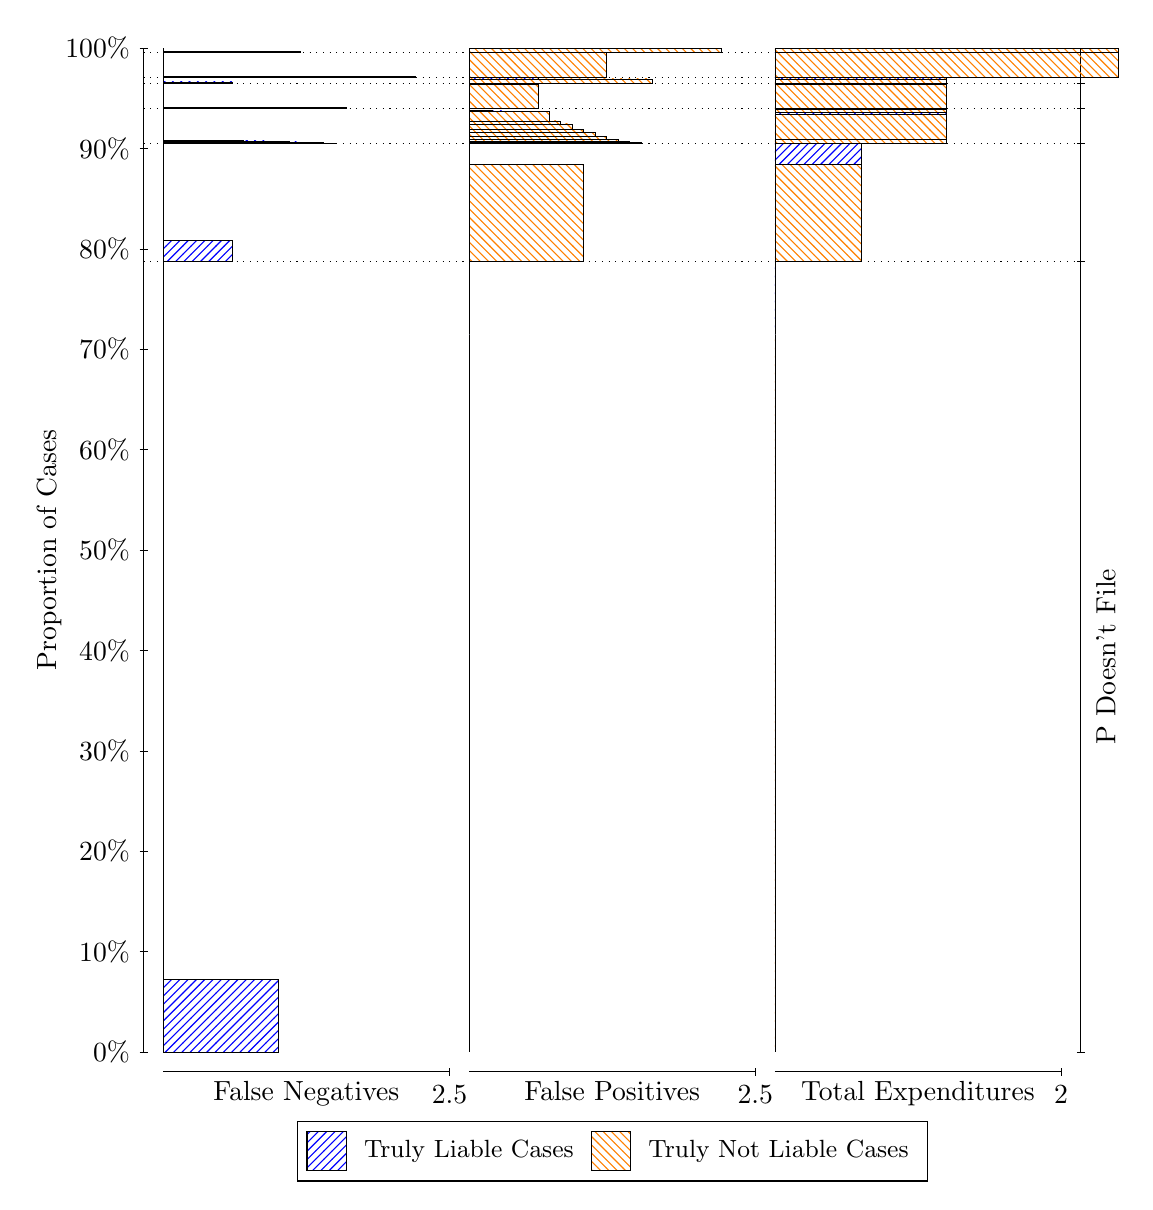
\begin{tikzpicture}
\draw[black, very thin] (1.5,1.75) -- (1.5,14.5);
\node[rotate=90, text=black, anchor=center] at (0.3, 8.125) {Proportion of Cases};
\draw[black, very thin] (1.45,1.75) -- (1.55,1.75);
\node[text=black, anchor=east] at (1.45, 1.75) {0\%};
\draw[black, very thin] (1.45,3.025) -- (1.55,3.025);
\node[text=black, anchor=east] at (1.45, 3.025) {10\%};
\draw[black, very thin] (1.45,4.3) -- (1.55,4.3);
\node[text=black, anchor=east] at (1.45, 4.3) {20\%};
\draw[black, very thin] (1.45,5.575) -- (1.55,5.575);
\node[text=black, anchor=east] at (1.45, 5.575) {30\%};
\draw[black, very thin] (1.45,6.85) -- (1.55,6.85);
\node[text=black, anchor=east] at (1.45, 6.85) {40\%};
\draw[black, very thin] (1.45,8.125) -- (1.55,8.125);
\node[text=black, anchor=east] at (1.45, 8.125) {50\%};
\draw[black, very thin] (1.45,9.4) -- (1.55,9.4);
\node[text=black, anchor=east] at (1.45, 9.4) {60\%};
\draw[black, very thin] (1.45,10.675) -- (1.55,10.675);
\node[text=black, anchor=east] at (1.45, 10.675) {70\%};
\draw[black, very thin] (1.45,11.95) -- (1.55,11.95);
\node[text=black, anchor=east] at (1.45, 11.95) {80\%};
\draw[black, very thin] (1.45,13.225) -- (1.55,13.225);
\node[text=black, anchor=east] at (1.45, 13.225) {90\%};
\draw[black, very thin] (1.45,14.5) -- (1.55,14.5);
\node[text=black, anchor=east] at (1.45, 14.5) {100\%};

\draw[black, very thin] (13.4,1.75) -- (13.4,14.5);
\draw[black, very thin] (13.35,1.75) -- (13.45,1.75);
\node[anchor=west] at (13.35, 1.75) {};
\draw[black, very thin] (13.35,11.789) -- (13.45,11.789);
\node[anchor=west] at (13.35, 11.789) {};
\draw[black, very thin] (13.35,13.288) -- (13.45,13.288);
\node[anchor=west] at (13.35, 13.288) {};
\draw[black, very thin] (13.35,13.732) -- (13.45,13.732);
\node[anchor=west] at (13.35, 13.732) {};
\draw[black, very thin] (13.35,14.05) -- (13.45,14.05);
\node[anchor=west] at (13.35, 14.05) {};
\draw[black, very thin] (13.35,14.129) -- (13.45,14.129);
\node[anchor=west] at (13.35, 14.129) {};
\draw[black, very thin] (13.35,14.446) -- (13.45,14.446);
\node[anchor=west] at (13.35, 14.446) {};
\draw[black, very thin] (13.35,14.5) -- (13.45,14.5);
\node[anchor=west] at (13.35, 14.5) {};

\draw[black, very thin, pattern color=blue, pattern=north east lines] (1.75,1.75) rectangle (3.2033,2.6747);
\draw[black, very thin, pattern color=orange, pattern=north west lines] (1.75,2.6747) rectangle (1.75,11.789);
\draw[black, very thin, pattern color=blue, pattern=north east lines] (1.75,11.789) rectangle (2.622,12.054);
\draw[black, very thin, pattern color=orange, pattern=north west lines] (1.75,12.054) rectangle (1.75,13.288);
\draw[black, very thin, pattern color=blue, pattern=north east lines] (1.75,13.288) rectangle (3.93,13.293);
\draw[black, very thin, pattern color=blue, pattern=north east lines] (1.75,13.293) rectangle (3.7847,13.297);
\draw[black, very thin, pattern color=blue, pattern=north east lines] (1.75,13.297) rectangle (3.6393,13.305);
\draw[black, very thin, pattern color=blue, pattern=north east lines] (1.75,13.305) rectangle (3.494,13.308);
\draw[black, very thin, pattern color=blue, pattern=north east lines] (1.75,13.308) rectangle (3.3487,13.314);
\draw[black, very thin, pattern color=blue, pattern=north east lines] (1.75,13.314) rectangle (3.2033,13.317);
\draw[black, very thin, pattern color=blue, pattern=north east lines] (1.75,13.317) rectangle (3.058,13.32);
\draw[black, very thin, pattern color=blue, pattern=north east lines] (1.75,13.32) rectangle (2.9127,13.322);
\draw[black, very thin, pattern color=blue, pattern=north east lines] (1.75,13.322) rectangle (2.7673,13.323);
\draw[black, very thin, pattern color=orange, pattern=north west lines] (1.75,13.323) rectangle (1.75,13.732);
\draw[black, very thin, pattern color=blue, pattern=north east lines] (1.75,13.732) rectangle (4.0753,13.748);
\draw[black, very thin, pattern color=orange, pattern=north west lines] (1.75,13.748) rectangle (1.75,14.05);
\draw[black, very thin, pattern color=blue, pattern=north east lines] (1.75,14.05) rectangle (2.622,14.071);
\draw[black, very thin, pattern color=orange, pattern=north west lines] (1.75,14.071) rectangle (1.75,14.129);
\draw[black, very thin, pattern color=blue, pattern=north east lines] (1.75,14.129) rectangle (4.9473,14.135);
\draw[black, very thin, pattern color=orange, pattern=north west lines] (1.75,14.135) rectangle (1.75,14.446);
\draw[black, very thin, pattern color=blue, pattern=north east lines] (1.75,14.446) rectangle (3.494,14.453);
\draw[black, very thin, pattern color=orange, pattern=north west lines] (1.75,14.453) rectangle (1.75,14.5);
\draw[black, very thin, pattern color=orange, pattern=north west lines] (5.6333,1.75) rectangle (5.6333,10.864);
\draw[black, very thin, pattern color=blue, pattern=north east lines] (5.6333,10.864) rectangle (5.6333,11.789);
\draw[black, very thin, pattern color=orange, pattern=north west lines] (5.6333,11.789) rectangle (7.0867,13.023);
\draw[black, very thin, pattern color=blue, pattern=north east lines] (5.6333,13.023) rectangle (5.6333,13.288);
\draw[black, very thin, pattern color=orange, pattern=north west lines] (5.6333,13.288) rectangle (7.8133,13.302);
\draw[black, very thin, pattern color=orange, pattern=north west lines] (5.6333,13.302) rectangle (7.668,13.316);
\draw[black, very thin, pattern color=orange, pattern=north west lines] (5.6333,13.316) rectangle (7.5227,13.344);
\draw[black, very thin, pattern color=orange, pattern=north west lines] (5.6333,13.344) rectangle (7.3773,13.38);
\draw[black, very thin, pattern color=orange, pattern=north west lines] (5.6333,13.38) rectangle (7.232,13.429);
\draw[black, very thin, pattern color=orange, pattern=north west lines] (5.6333,13.429) rectangle (7.0867,13.464);
\draw[black, very thin, pattern color=orange, pattern=north west lines] (5.6333,13.464) rectangle (6.9413,13.537);
\draw[black, very thin, pattern color=orange, pattern=north west lines] (5.6333,13.537) rectangle (6.796,13.576);
\draw[black, very thin, pattern color=orange, pattern=north west lines] (5.6333,13.576) rectangle (6.6507,13.697);
\draw[black, very thin, pattern color=blue, pattern=north east lines] (5.6333,13.697) rectangle (6.36,13.698);
\draw[black, very thin, pattern color=blue, pattern=north east lines] (5.6333,13.698) rectangle (6.2147,13.699);
\draw[black, very thin, pattern color=blue, pattern=north east lines] (5.6333,13.699) rectangle (6.0693,13.702);
\draw[black, very thin, pattern color=blue, pattern=north east lines] (5.6333,13.702) rectangle (5.924,13.706);
\draw[black, very thin, pattern color=blue, pattern=north east lines] (5.6333,13.706) rectangle (5.7787,13.711);
\draw[black, very thin, pattern color=blue, pattern=north east lines] (5.6333,13.711) rectangle (5.6333,13.732);
\draw[black, very thin, pattern color=orange, pattern=north west lines] (5.6333,13.732) rectangle (6.5053,14.034);
\draw[black, very thin, pattern color=blue, pattern=north east lines] (5.6333,14.034) rectangle (5.6333,14.05);
\draw[black, very thin, pattern color=orange, pattern=north west lines] (5.6333,14.05) rectangle (7.9587,14.108);
\draw[black, very thin, pattern color=blue, pattern=north east lines] (5.6333,14.108) rectangle (6.5053,14.129);
\draw[black, very thin, pattern color=orange, pattern=north west lines] (5.6333,14.129) rectangle (7.3773,14.44);
\draw[black, very thin, pattern color=blue, pattern=north east lines] (5.6333,14.44) rectangle (5.924,14.446);
\draw[black, very thin, pattern color=orange, pattern=north west lines] (5.6333,14.446) rectangle (8.8307,14.492);
\draw[black, very thin, pattern color=blue, pattern=north east lines] (5.6333,14.492) rectangle (7.3773,14.5);
\draw[black, very thin, pattern color=orange, pattern=north west lines] (9.5167,1.75) rectangle (9.5167,10.864);
\draw[black, very thin, pattern color=blue, pattern=north east lines] (9.5167,10.864) rectangle (9.5167,11.789);
\draw[black, very thin, pattern color=orange, pattern=north west lines] (9.5167,11.789) rectangle (10.607,13.023);
\draw[black, very thin, pattern color=blue, pattern=north east lines] (9.5167,13.023) rectangle (10.607,13.288);
\draw[black, very thin, pattern color=orange, pattern=north west lines] (9.5167,13.288) rectangle (11.697,13.337);
\draw[black, very thin, pattern color=blue, pattern=north east lines] (9.5167,13.337) rectangle (11.697,13.343);
\draw[black, very thin, pattern color=orange, pattern=north west lines] (9.5167,13.343) rectangle (11.697,13.659);
\draw[black, very thin, pattern color=blue, pattern=north east lines] (9.5167,13.659) rectangle (11.697,13.685);
\draw[black, very thin, pattern color=orange, pattern=north west lines] (9.5167,13.685) rectangle (11.697,13.727);
\draw[black, very thin, pattern color=blue, pattern=north east lines] (9.5167,13.727) rectangle (11.697,13.732);
\draw[black, very thin, pattern color=orange, pattern=north west lines] (9.5167,13.732) rectangle (11.697,14.034);
\draw[black, very thin, pattern color=blue, pattern=north east lines] (9.5167,14.034) rectangle (11.697,14.05);
\draw[black, very thin, pattern color=orange, pattern=north west lines] (9.5167,14.05) rectangle (11.697,14.108);
\draw[black, very thin, pattern color=blue, pattern=north east lines] (9.5167,14.108) rectangle (11.697,14.129);
\draw[black, very thin, pattern color=orange, pattern=north west lines] (9.5167,14.129) rectangle (13.877,14.44);
\draw[black, very thin, pattern color=blue, pattern=north east lines] (9.5167,14.44) rectangle (13.877,14.446);
\draw[black, very thin, pattern color=orange, pattern=north west lines] (9.5167,14.446) rectangle (13.877,14.492);
\draw[black, very thin, pattern color=blue, pattern=north east lines] (9.5167,14.492) rectangle (13.877,14.5);
\draw[black, dotted] (1.5,11.789) -- (13.4,11.789);
\draw[black, dotted] (1.5,13.288) -- (13.4,13.288);
\draw[black, dotted] (1.5,13.732) -- (13.4,13.732);
\draw[black, dotted] (1.5,14.05) -- (13.4,14.05);
\draw[black, dotted] (1.5,14.129) -- (13.4,14.129);
\draw[black, dotted] (1.5,14.446) -- (13.4,14.446);
\draw[black, very thin] (1.75,1.5) -- (5.3833,1.5);
\node[text=black, anchor=north] at (3.5667, 1.5) {False Negatives};
\draw[black, very thin] (5.3833,1.45) -- (5.3833,1.55);
\node[text=black, anchor=north] at (5.3833, 1.45) {2.5};

\draw[black, very thin] (5.6333,1.5) -- (9.2667,1.5);
\node[text=black, anchor=north] at (7.45, 1.5) {False Positives};
\draw[black, very thin] (9.2667,1.45) -- (9.2667,1.55);
\node[text=black, anchor=north] at (9.2667, 1.45) {2.5};

\draw[black, very thin] (9.5167,1.5) -- (13.15,1.5);
\node[text=black, anchor=north] at (11.333, 1.5) {Total Expenditures};
\draw[black, very thin] (13.15,1.45) -- (13.15,1.55);
\node[text=black, anchor=north] at (13.15, 1.45) {2};

\node[text=black, centered, rotate=90] at (13.72, 6.7695) {P Doesn't File};







\draw (7.449999999999999,1.5) node[draw=none] (baseCoordinate) {};
\begin{scope}[align=center]
        \matrix[scale=0.5, draw=black, below=0.5cm of baseCoordinate, nodes={draw}, column sep=0.1cm]{
            \node[rectangle, draw, minimum width=0.5cm, minimum height=0.5cm, pattern color=blue, pattern=north east lines] {}; &
            \node[draw=none, font=\small, text=black] (B) {Truly Liable Cases}; &
            \node[rectangle, draw, minimum width=0.5cm, minimum height=0.5cm, pattern color=orange, pattern=north west lines] {}; &
            \node[draw=none, font=\small, text=black] (B) {Truly Not Liable Cases}; \\
            };
\end{scope}

\end{tikzpicture}
\end{document}